\chapter{Agentes especializados y meta-agente}
\label{chap:agentes}

Este capítulo describe la parte propiamente predictiva del sistema. La hipótesis no es que una sola
familia de ratios domine de forma estable todos los regímenes, sino que distintas vistas económicas
del universo aportan información con persistencia desigual. Por ello se entrenan cinco agentes
especializados ---\textit{quality}, \textit{value}, \textit{growth}, \textit{momentum} y
\textit{risk}--- y un combinador que aprende cómo ponderarlos sin conocer a priori cuál será el
más útil.

\section{Arquitectura y aprendizaje \textit{walk-forward}}

Cada agente recibe sólo los bloques de variables asignados a su especialidad. \textit{Quality}
resume rentabilidad, márgenes, eficiencia y solidez financiera; \textit{value} utiliza ratios de
precio y flujos; \textit{growth} mide aceleración y estabilidad de fundamentales; \textit{momentum}
recoge tendencias de precio y de fundamentales; y \textit{risk} representa riesgo de precio y
liquidez. Esta separación tiene dos fines: conserva interpretabilidad económica y evita que el
meta-agente confunda cinco copias del mismo predictor.

En cada fecha de snapshot se ajusta un LightGBM por agente sobre una ventana móvil de ocho años.
El ganador fijado por el estudio emplea profundidad máxima 3, 100 estimadores, tasa de aprendizaje
0,03 y mínimo de 50 observaciones por hoja. LightGBM permite representar interacciones no lineales
sin imponer una forma funcional única (Ke et al., 2017); el entrenamiento temporal evita
que el modelo evalúe observaciones que habría visto durante el ajuste.

Las cinco puntuaciones se convierten en rangos transversales y pasan al meta-agente. El catálogo
ofrece dos variantes y la configuración ganadora emplea \texttt{stacked\_rolling\_free}: usa
exclusivamente cohortes trimestrales cerradas de los trimestres precedentes y estima una Ridge
positiva \emph{sin} tope por agente. Si todavía no hay etiquetas cerradas suficientes, usa por
construcción pesos iguales de 0,20.

La alternativa \texttt{stacked\_rolling\_bounded}, que acota los pesos entre 0,10 y 0,50, fue la que
emplearon las dos primeras pasadas de la cadena. Su restricción superior era deliberada: impedía que
una ventaja transitoria apagase por completo a los restantes agentes. La tercera pasada la sustituyó
por la variante libre porque medía mejor en Rank-IC, y la consecuencia de esa decisión --- un
reparto final casi degenerado --- se analiza más adelante en este capítulo.

\begin{figure}[H]
  \centering
  \begin{tikzpicture}[node distance=9mm and 12mm, >=Latex, every node/.style={font=\small}]
    \node[draw,rounded corners,fill=blue!8,minimum width=25mm,minimum height=10mm] (f) {Variables PIT};
    \node[draw,rounded corners,fill=teal!10,right=of f,minimum width=31mm,minimum height=22mm,align=center] (a) {Cinco agentes\\LightGBM};
    \node[draw,rounded corners,fill=orange!12,right=of a,minimum width=32mm,minimum height=16mm,align=center] (m) {Meta apilado\\acotado};
    \node[draw,rounded corners,fill=green!10,right=of m,minimum width=26mm,minimum height=10mm,align=center] (s) {Ranking final};
    \draw[->,thick] (f) -- (a);
    \draw[->,thick] (a) -- (m);
    \draw[->,thick] (m) -- (s);
  \end{tikzpicture}
  \caption{Arquitectura predictiva. Las variables sólo están disponibles cuando ya se publicaron;
  los agentes se ajustan \textit{walk-forward} y el meta aprende con cohortes cuya etiqueta ya cerró.}
  \label{fig:arquitectura}
\end{figure}

\section{La evidencia de que el meta aprende}

El aprendizaje es observable, no una afirmación inferida de la rentabilidad final. Las primeras
filas de \texttt{meta\_weights.parquet} corresponden a \texttt{fallback\_equal}: cada agente recibe
0,20 porque aún no existe evidencia cerrada. Después aparecen las filas \texttt{learned}, y en ellas
el peso de \textit{risk} crece de forma sostenida a medida que se cierran cohortes: 0,22 de media en
2016, 0,45 en 2017, 0,66 en 2018, 0,83 en 2020 y valores en torno a 0,95 desde 2022. Al final de la
serie el reparto es prácticamente degenerado --- 0,954 para \textit{risk} y 0,047 para
\textit{value}, con los tres agentes restantes en cero ---, de modo que el meta-agente no aprendió a
combinar cinco especialistas sino a descartar cuatro.

Ese desenlace merece leerse con cuidado, porque es el resultado esperable del método y no una
anomalía. La configuración ganadora emplea \texttt{stacked\_rolling\_free}, es decir, un apilado sin
tope por agente; enfrentado a un especialista que domina de forma consistente, el procedimiento
converge a él. Las pasadas anteriores de la cadena usaban la variante acotada, y el cambio a la
libre fue precisamente la única decisión que la tercera pasada modificó. Se ganó Rank-IC ---
$+0{,}00827$ de ventaja pareada --- a costa de que la arquitectura multi-agente quede, en la
práctica, reducida a uno.

\begin{figure}[H]
  \centering
  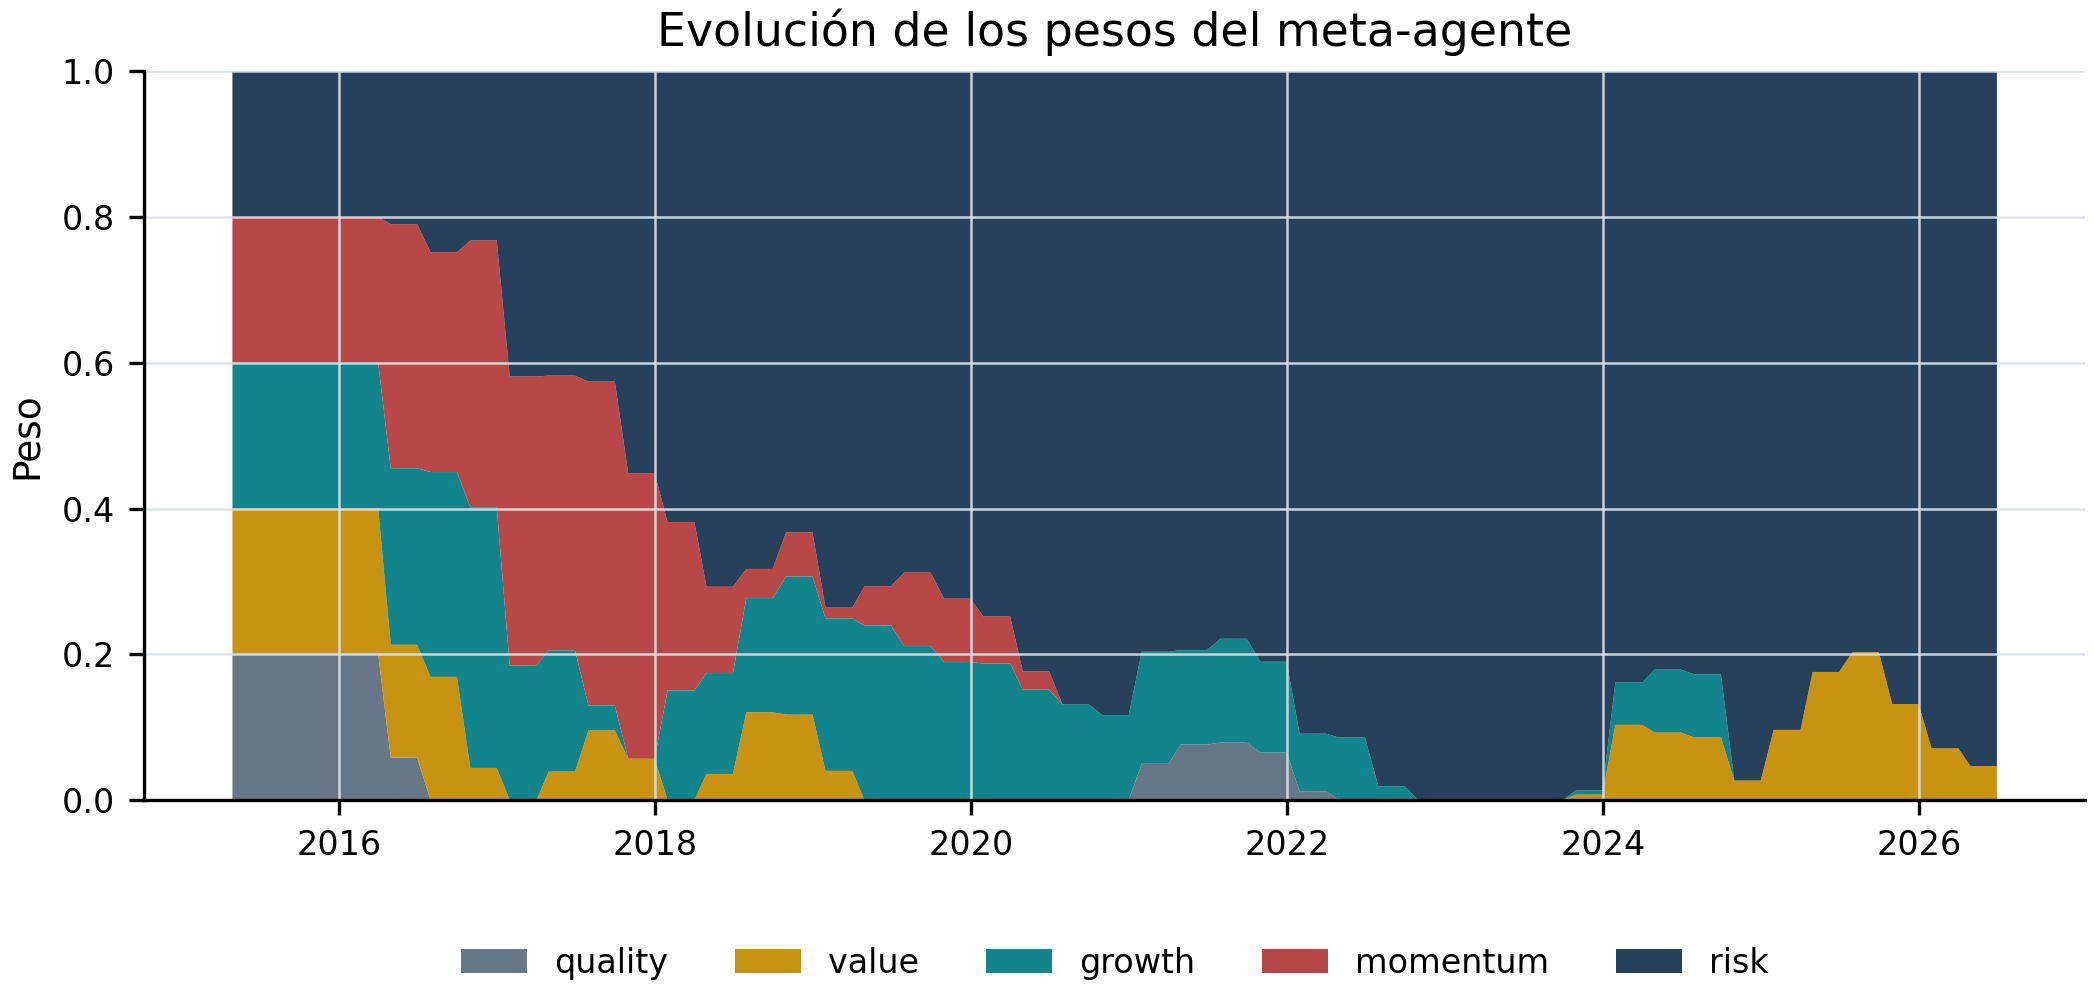
\includegraphics[width=0.94\textwidth]{assets/f05_meta_pesos.png}
  \caption{Pesos del meta-agente por fecha de snapshot. La franja inicial uniforme corresponde a
  la ausencia de etiquetas cerradas; las variaciones posteriores usan únicamente información ya
  observable. Fuente: \texttt{evidence/meta\_weights.parquet}.}
  \label{fig:pesos-meta}
\end{figure}

El contraste relevante conserva exactamente los mismos cinco agentes y cambia sólo la regla de
combinación. En la ventana de selección, el meta aprendido alcanza Rank-IC 0,1090 frente a 0,0675
del promedio equiponderado: una mejora de 0,0415, equivalente al 61\%. Por tanto, la capa de
combinación añade información útil y no sólo reescala los scores.

Hay, sin embargo, un resultado que este trabajo debe reportar aunque incomode a su propia
arquitectura: \textbf{el agente \textit{risk} por separado ordena mejor que el meta-agente}. Su
Rank-IC en la ventana de selección es 0,1227 con IC-IR 0,988 y 80,34\% de cohortes positivas, frente
a 0,1090, 0,851 y 74,36\% del meta. La diferencia es pequeña, pero va en la dirección contraria a la
que justificaría la complejidad añadida.

La explicación es coherente con lo anterior. El meta-agente converge hacia \textit{risk} pero tarda
años en hacerlo, y durante ese trayecto arrastra el peso de agentes que ordenan mucho peor ---
\textit{quality} 0,0096 y \textit{momentum} 0,0005, ambos indistinguibles de cero. Su ventaja frente
al reparto uniforme es real y grande; su desventaja frente al mejor especialista aislado también lo
es. La lectura honesta es que el meta-agente demuestra saber \emph{aprender} de la evidencia, pero
no que combinar aporte más que seleccionar bien, y el documento no presenta la arquitectura
multi-agente como demostrada por estos datos. Debe añadirse un matiz que impide cerrar la cuestión
en sentido contrario: la superioridad de \textit{risk} se conoce \emph{a posteriori}, mirando la
ventana completa, mientras que el meta la descubrió progresivamente y sin usar información futura.
Elegir \textit{risk} de antemano no era una opción disponible en 2015.

\begin{table}[H]
  \centering
  \caption{Capacidad predictiva de los agentes y combinadores en 2015--2024.}
  \label{tab:agentes}
  \begin{tabular}{lrrrr}
\toprule
Señal & Rank-IC & Desv. & Positivas & IC-IR \\
\midrule
risk & 0,1227 & 0,1241 & 80,34\% & 0,988 \\
meta\_final & 0,1090 & 0,1281 & 74,36\% & 0,851 \\
meta\_equal\_weight & 0,0675 & 0,1261 & 62,39\% & 0,535 \\
growth & 0,0249 & 0,0865 & 61,54\% & 0,289 \\
value & 0,0244 & 0,0803 & 63,25\% & 0,303 \\
quality & 0,0096 & 0,1051 & 47,01\% & 0,091 \\
momentum & 0,0005 & 0,0902 & 47,86\% & 0,006 \\
\bottomrule
\end{tabular}

  \caption*{Fuente: \texttt{evidence/rank\_ic\_diagnostics.parquet}. Desviación e IC-IR se calculan
  sobre cohortes cerradas de la ventana de selección.}
\end{table}

\begin{figure}[H]
  \centering
  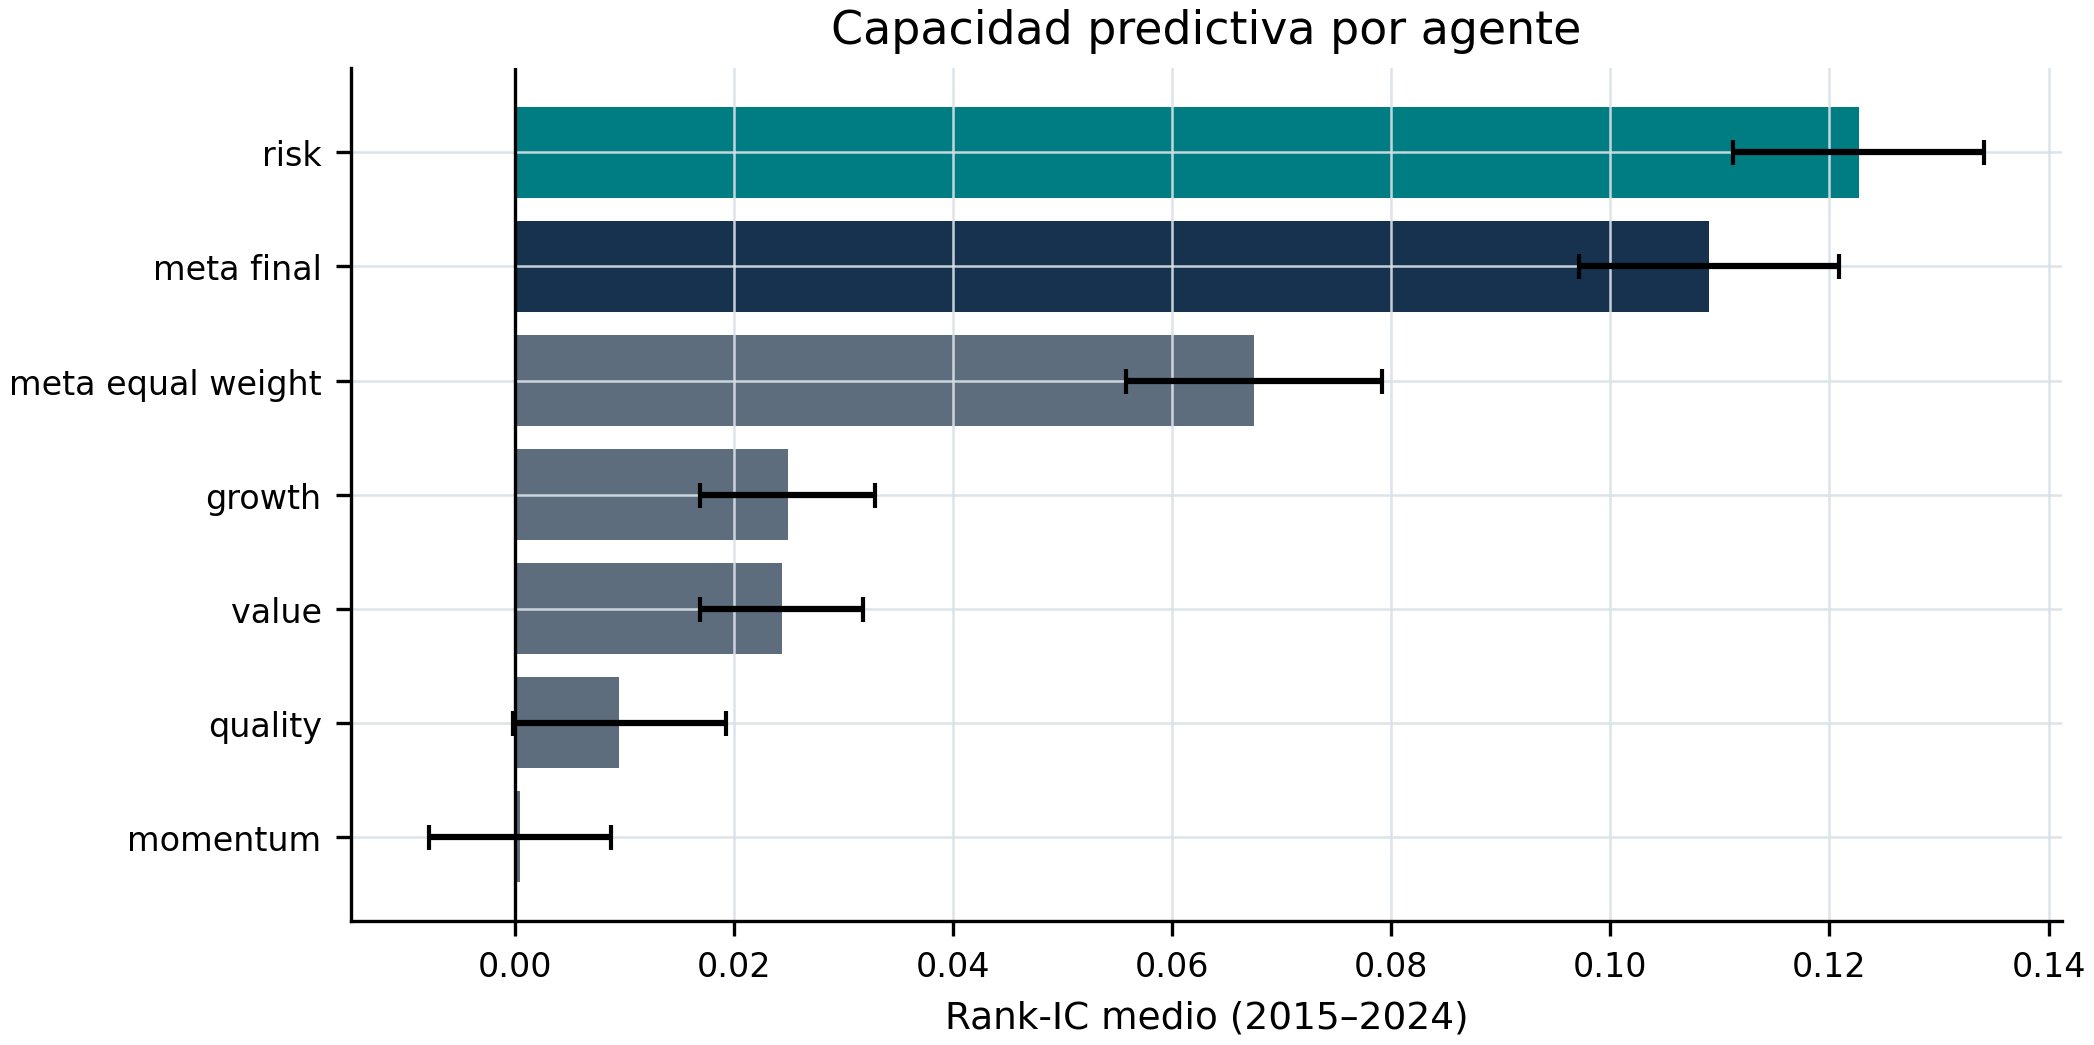
\includegraphics[width=0.90\textwidth]{assets/f05_agentes_rankic.png}
  \caption{Rank-IC medio por señal; las barras de error muestran el error estándar de la media.
  Fuente: \texttt{evidence/rank\_ic\_diagnostics.parquet}.}
  \label{fig:agentes-rankic}
\end{figure}

Hay un matiz esencial. \textit{Risk} aislado presenta el mayor Rank-IC: 0,1227, por encima del
0,1090 del meta. La conclusión defendible no es que el meta supere a su mejor componente, sino que
aprende desde una situación de ignorancia a superar con claridad la combinación ingenua y a
reproducir casi toda la señal del especialista dominante sin conocerlo de antemano. El
Capítulo~\ref{chap:resultados} comprobará además que dicha señal conserva el 86,62\% tras
neutralizar controles de estilo, de modo que no debe reducirse sin más a baja volatilidad clásica.

Conviene una advertencia de lectura que afecta a todo el capítulo. Los artefactos contienen dos
ventanas distintas para esta misma métrica: la de \emph{selección}, con 117 cohortes hasta 2024, y
la \emph{completa}, con 123 cohortes que incluyen las cerradas de la era reservada. En la primera,
\textit{risk} obtiene 0,1227 y el meta 0,1090; en la segunda, 0,1197 y 0,1058. Ninguna es más
correcta que la otra, pero mezclarlas produce discrepancias aparentes. Las tablas de este capítulo
usan la ventana de selección salvo indicación expresa.

\subsection*{Estabilidad por eras: qué aprendió y qué no}

Una media agregada puede ocultar que una señal funcionó en un régimen y no en otro. La
Tabla~\ref{tab:rankic-era} y la Figura~\ref{fig:rankic-era} descomponen el Rank-IC de cada señal por
era, incluyendo la reservada a título informativo.

\begin{table}[H]
  \centering
  \small
  \caption{Rank-IC medio por señal y era.}
  \label{tab:rankic-era}
  \begin{tabular}{lrrrr}
\toprule
Señal & 2015-2018 & 2019-2021 & 2022-2024 & 2025-2026 \\
\midrule
risk & 0,1238 & 0,0577 & 0,1778 & 0,0669 \\
meta final & 0,0949 & 0,0543 & 0,1739 & 0,0364 \\
meta equal weight & 0,0811 & 0,0184 & 0,1045 & -0,0868 \\
value & 0,0205 & 0,0330 & 0,0347 & -0,1284 \\
growth & 0,0493 & 0,0193 & 0,0137 & -0,1476 \\
quality & 0,0018 & -0,0110 & 0,0399 & -0,0533 \\
momentum & 0,0331 & -0,0450 & 0,0019 & -0,0009 \\
\bottomrule
\end{tabular}

  \caption*{Fuente: \artefacto{evidence/rank\_ic\_diagnostics.parquet}. Las tres primeras columnas
  son ventana de selección; la cuarta es la era reservada y no intervino en ninguna decisión.}
\end{table}

\begin{figure}[H]
  \centering
  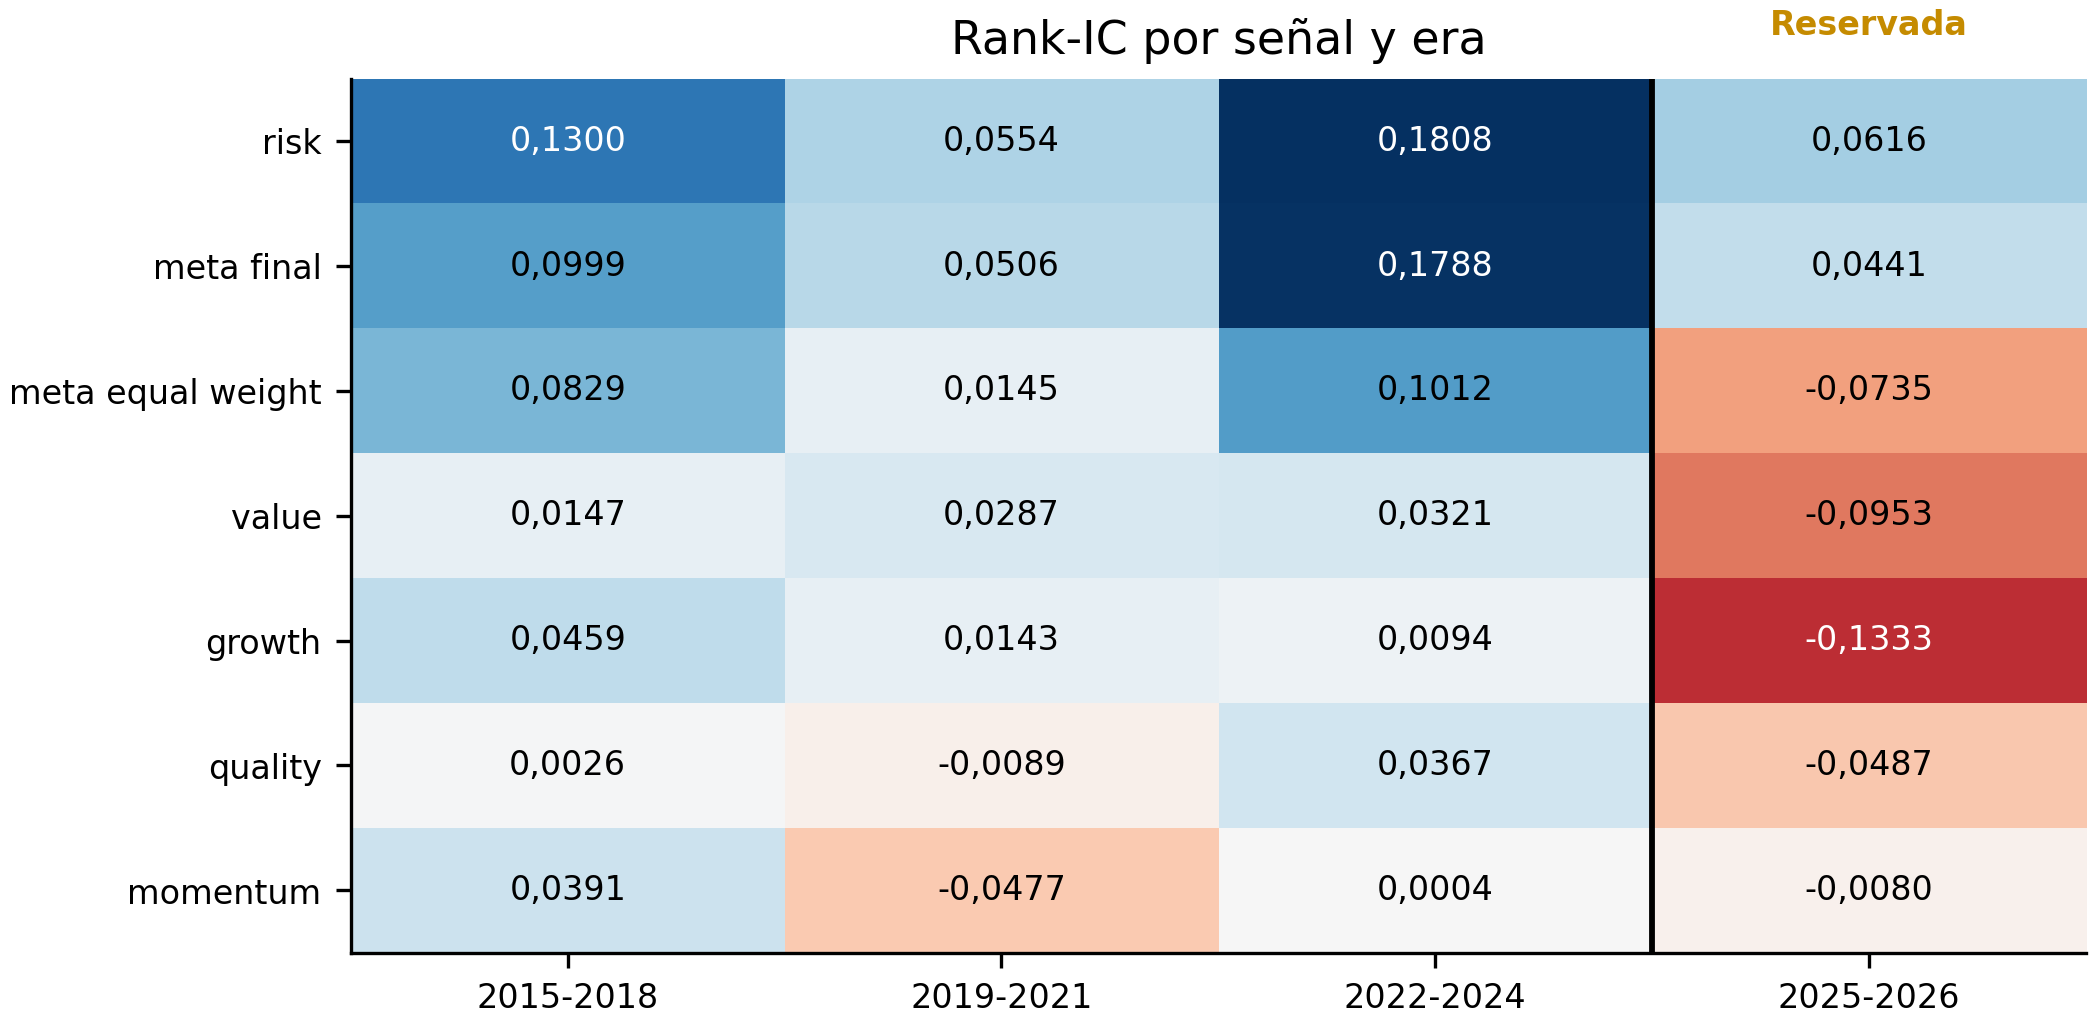
\includegraphics[width=0.94\textwidth]{assets/f05_rankic_era.png}
  \caption{Rank-IC por señal y era. El azul indica capacidad predictiva positiva y el rojo negativa;
  la línea vertical separa la era reservada. Fuente:
  \artefacto{evidence/rank\_ic\_diagnostics.parquet}.}
  \label{fig:rankic-era}
\end{figure}

La tabla contiene tres lecturas que el promedio agregado no permite. La primera es que \textit{risk}
es la única señal positiva en las cuatro eras; ninguna otra lo consigue. La segunda es que el meta
aprendido supera al equiponderado en las tres eras de selección, no sólo en promedio, lo que
refuerza que la mejora del 52\,\% no procede de un único subperiodo afortunado. La tercera es la más
incómoda y se reporta precisamente por serlo: en la era reservada todos los agentes fundamentales se
vuelven negativos a la vez --- \textit{growth} llega a $-0{,}1352$ --- y sólo \textit{risk} aguanta
en positivo. El meta queda en $-0{,}0119$, prácticamente en cero.

Que los cinco agentes se inviertan simultáneamente es informativo: apunta a una rotación de factores
en el mercado y no a un error de signo en un modelo concreto, que afectaría a uno solo. Este mismo
patrón fue el que motivó introducir la ponderación por recencia como variable del catálogo, según se
documenta en el Capítulo~\ref{chap:desarrollo-metodo}. Debe leerse junto a la advertencia estadística del
Capítulo~\ref{chap:resultados}: son seis cohortes cerradas y una observación independiente efectiva,
insuficiente para concluir que la capacidad predictiva se haya degradado.

\subsection*{La trayectoria del peso aprendido}

La Tabla~\ref{tab:pesos-anual} y la Figura~\ref{fig:pesos-anual} muestran cómo evoluciona la
ponderación año a año.

\begin{table}[H]
  \centering
  \small
  \caption{Peso medio anual asignado por el meta-agente a cada especialista.}
  \label{tab:pesos-anual}
  \begin{tabular}{lrrrrrl}
\toprule
Año & risk & growth & momentum & quality & value & Estado \\
\midrule
2015 & 0,200 & 0,200 & 0,200 & 0,200 & 0,200 & uniforme \\
2016 & 0,203 & 0,263 & 0,281 & 0,125 & 0,128 & aprendido \\
2017 & 0,370 & 0,116 & 0,315 & 0,100 & 0,100 & aprendido \\
2018 & 0,493 & 0,170 & 0,130 & 0,104 & 0,104 & aprendido \\
2019 & 0,490 & 0,210 & 0,100 & 0,100 & 0,100 & aprendido \\
2020 & 0,500 & 0,172 & 0,109 & 0,109 & 0,109 & aprendido \\
2021 & 0,500 & 0,188 & 0,104 & 0,104 & 0,104 & aprendido \\
2022 & 0,500 & 0,128 & 0,124 & 0,124 & 0,124 & aprendido \\
2023 & 0,500 & 0,125 & 0,125 & 0,125 & 0,125 & aprendido \\
2024 & 0,500 & 0,126 & 0,125 & 0,125 & 0,125 & aprendido \\
2025 & 0,500 & 0,114 & 0,114 & 0,114 & 0,159 & aprendido \\
2026 & 0,500 & 0,125 & 0,125 & 0,125 & 0,125 & aprendido \\
\bottomrule
\end{tabular}

  \caption*{Fuente: \artefacto{evidence/meta\_weights.parquet}. 2015 corresponde íntegramente al
  reparto uniforme por ausencia de cohortes cerradas.}
\end{table}

\begin{figure}[H]
  \centering
  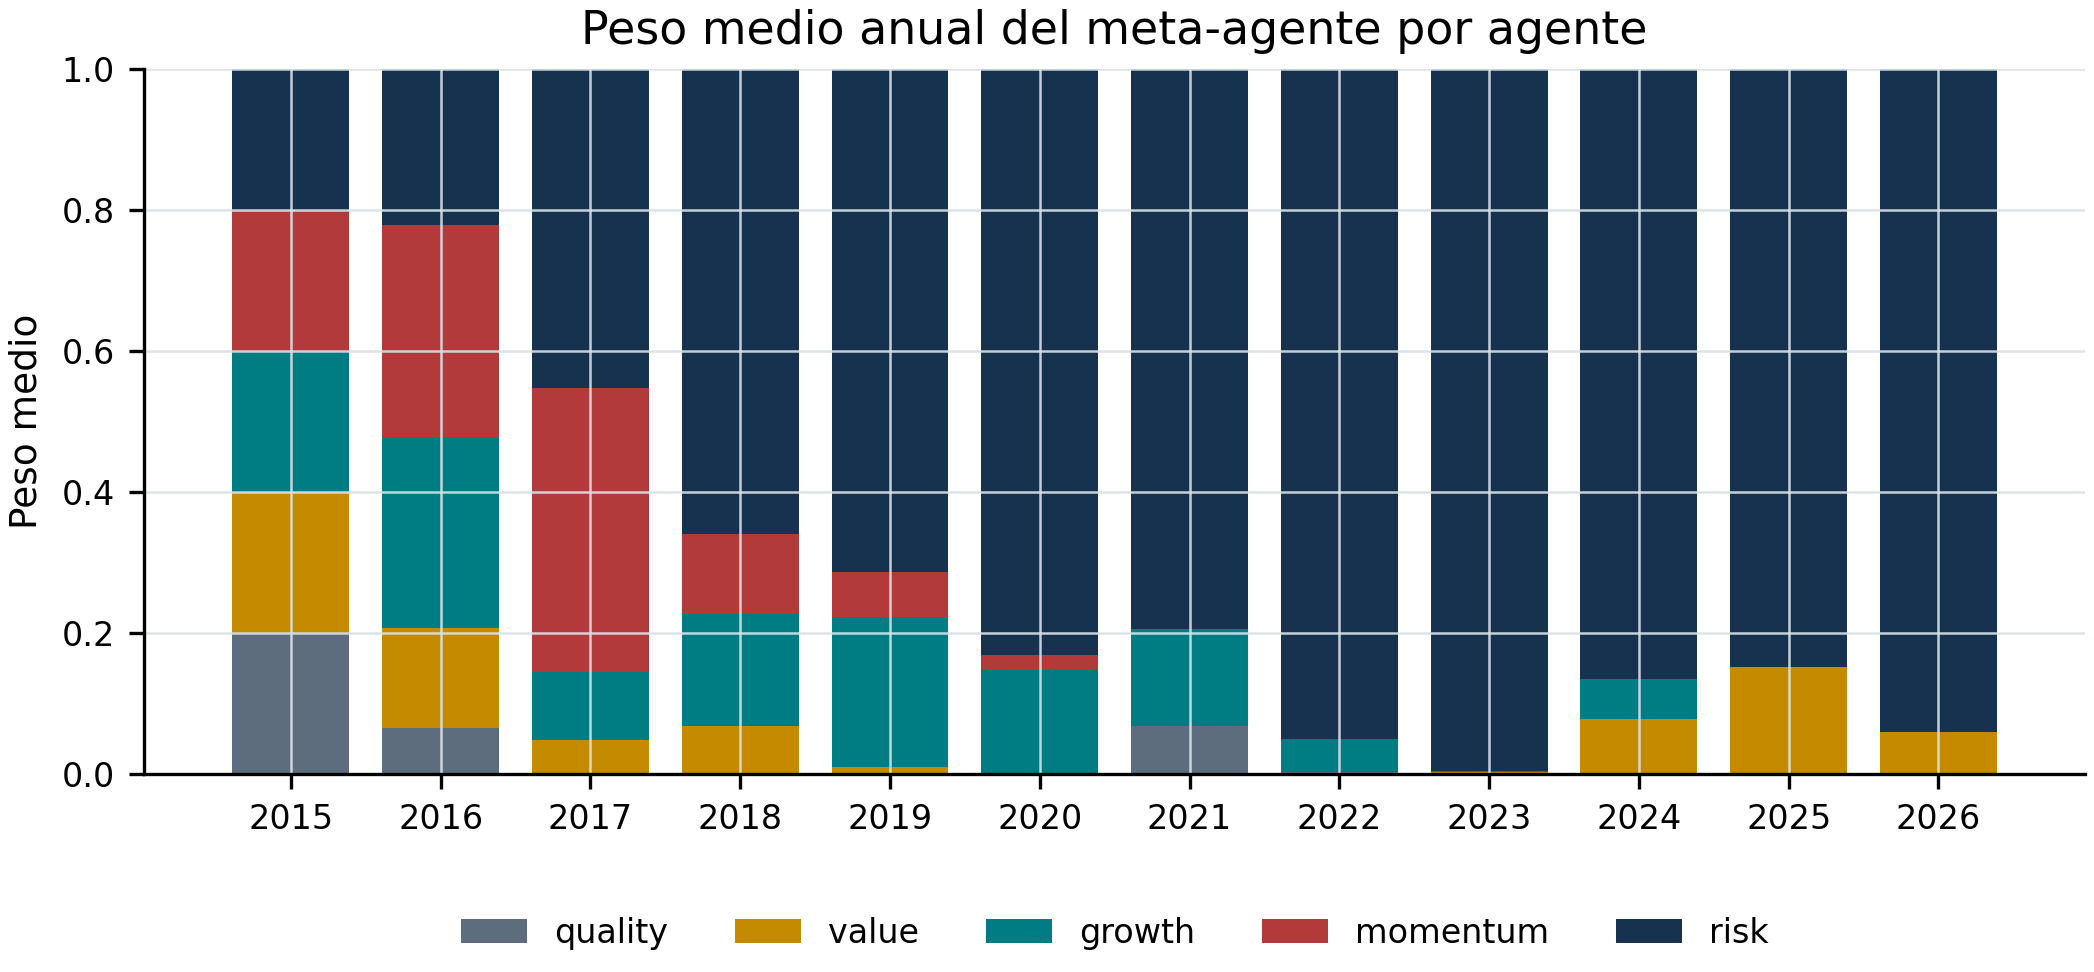
\includegraphics[width=0.94\textwidth]{assets/f05_pesos_anual.png}
  \caption{Peso medio anual por agente. Fuente: \artefacto{evidence/meta\_weights.parquet}.}
  \label{fig:pesos-anual}
\end{figure}

La trayectoria describe un aprendizaje reconocible. En 2015 el reparto es uniforme por construcción,
al no existir evidencia cerrada. En 2016 el meta concentra en \textit{momentum}, que acabará siendo
el peor especialista de todo el periodo: es un error, y es exactamente lo que cabe esperar de un
sistema que decide con dos años de datos. En 2017 corrige hacia \textit{risk} (0,45 de media anual),
en 2018 lo eleva a 0,66 y a partir de 2020 lo sitúa por encima de 0,83, alcanzando 0,997 en 2023.

\subsection*{Qué significa que el meta se concentre casi por completo}

Que el peso de \textit{risk} termine rozando la unidad es un resultado ambivalente y conviene no
presentarlo sólo por su lado favorable.

Leído a favor, demuestra que el aprendizaje funciona: el sistema identifica a su mejor especialista
en unos dos años, partiendo de la ignorancia, y mantiene esa identificación de forma estable en vez
de oscilar entre candidatos.

Leído en contra, significa que la arquitectura multi-agente se vacía de contenido en su propio
ganador. Un meta que asigna el 95\,\% del peso a un único agente ha dejado de ser un combinador para
ser un selector, y su comportamiento fuera de muestra depende por completo de que ese agente siga
funcionando. Las dos primeras pasadas de la cadena usaban una variante acotada, que impedía superar
0,50 precisamente para evitar este desenlace; la tercera adoptó la variante libre porque medía mejor
en Rank-IC. Es un caso claro de decisión que mejora la métrica de selección y empeora una propiedad
cualitativa del diseño que ninguna métrica del protocolo estaba midiendo.

Con la restricción levantada, la comparación entre el meta y \textit{risk} aislado ya no puede
atribuirse al tope: el meta puede concentrarse cuanto quiera y aun así ordena algo peor (0,1090
frente a 0,1227). La diferencia procede de los años iniciales, cuando todavía repartía peso entre
agentes que resultaron ser inútiles, y ese coste es irrecuperable porque forma parte de lo que
significa aprender sin mirar al futuro.

El riesgo que la restricción pretendía cubrir sigue existiendo, y ahora está asumido: la señal del
sistema es, en la práctica, la del agente \textit{risk}, de modo que su comportamiento futuro
depende de que ese especialista siga funcionando. La era reservada permite una primera comprobación
--- el Rank-IC se mantiene positivo en $+0{,}0441$ ---, pero seis cohortes no bastan para descartar
que la concentración sea frágil. Queda recogido como limitación en el
Capítulo~\ref{chap:limitaciones}.

\begin{figure}[H]
  \centering
  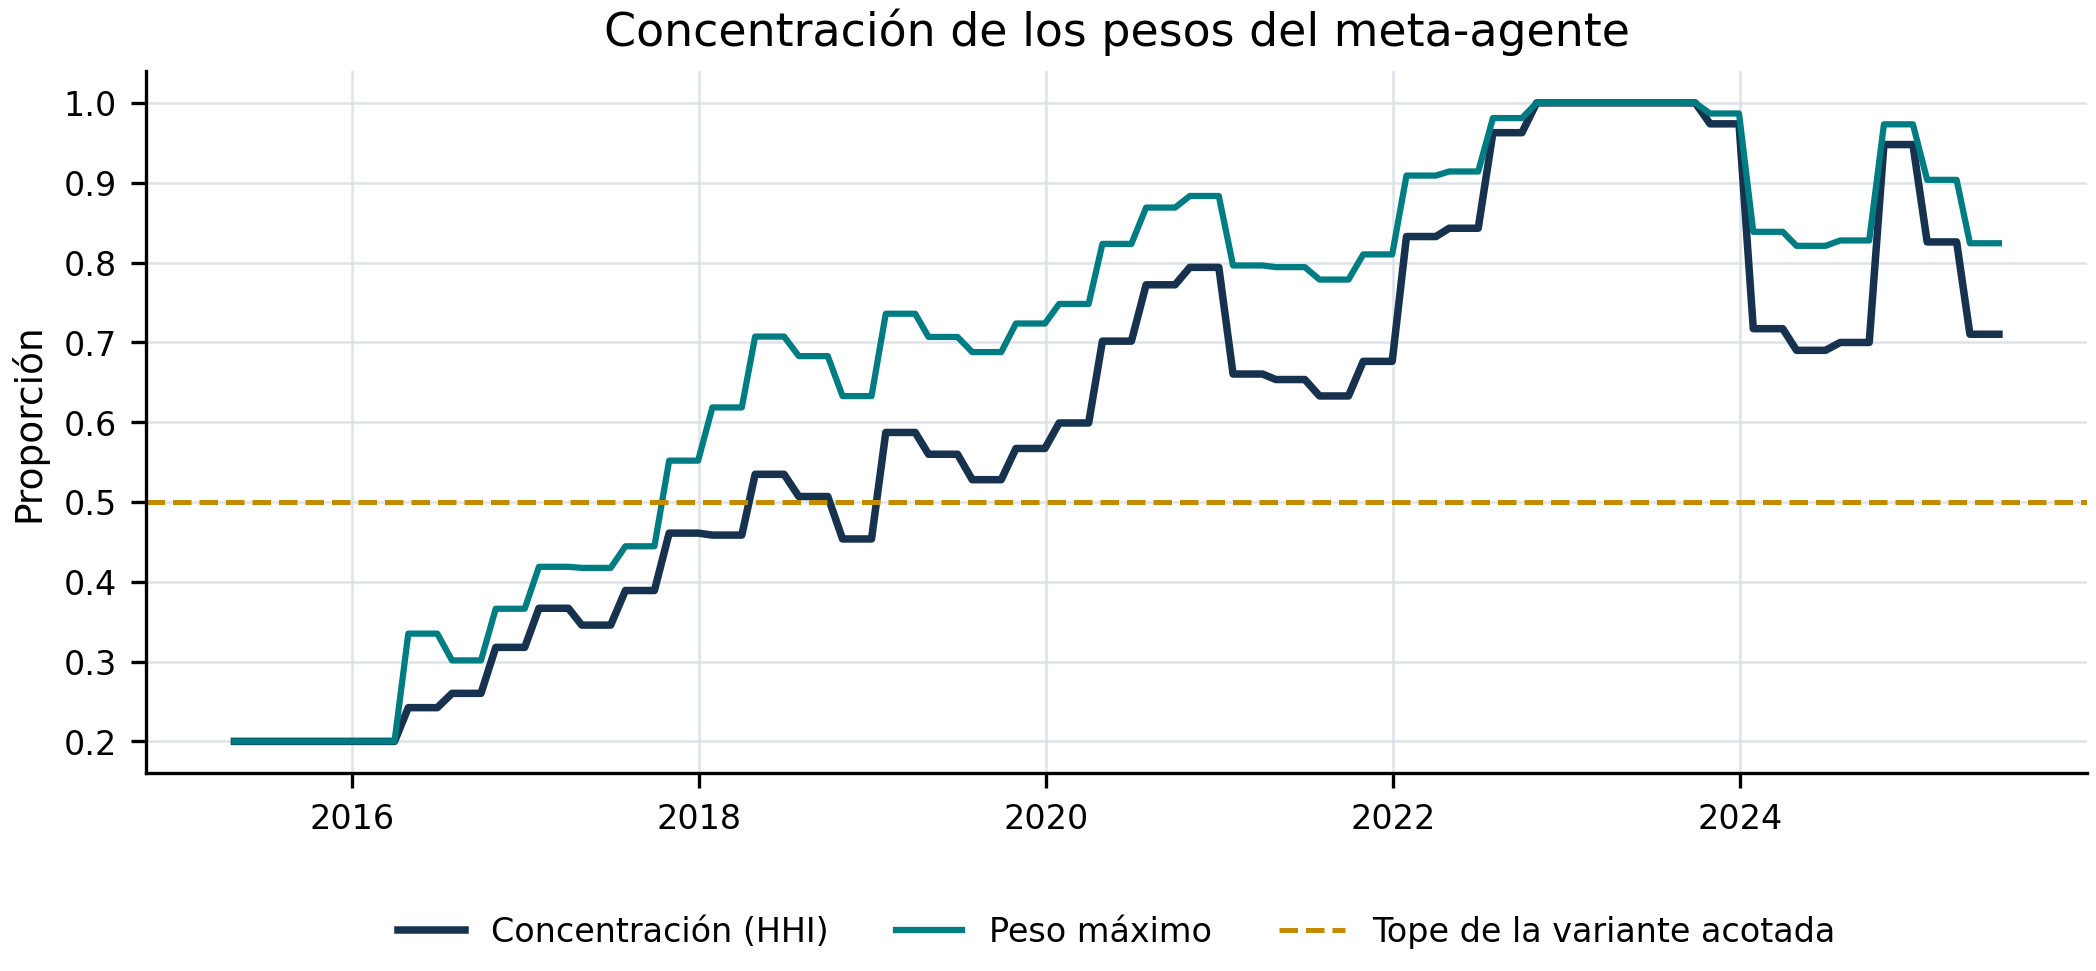
\includegraphics[width=0.94\textwidth]{assets/f05_concentracion.png}
  \caption{Concentración de los pesos del meta-agente y peso máximo asignado, por fecha. Fuente:
  \artefacto{evidence/rank\_tail\_diagnostics.parquet}.}
  \label{fig:concentracion}
\end{figure}

\section{Qué aprende cada especialista}

La especialización no asigna una conclusión previa al modelo; asigna un vocabulario económico para
formular hipótesis. El agente \textit{quality} recibe ratios como ROE, ROIC, ROA, márgenes, rotación
de activos, liquidez y endeudamiento. Un ROIC alto puede indicar un uso eficiente del capital, pero
el modelo no recibe la regla ``ROIC alto implica comprar''; aprende una relación condicionada a la
historia disponible. \textit{Value} combina valoraciones relativas y flujos de caja; \textit{growth}
busca aceleración, persistencia y estabilidad de resultados; \textit{momentum} incorpora tendencia
de precio y de fundamentales; y \textit{risk} resume volatilidad, riesgo de precio y liquidez.

El preset ganador, \texttt{all}, activa once bloques cerrados y conserva como máximo doce variables
por agente mediante poda por estabilidad fuera de muestra. Así evita un conjunto demasiado reducido,
que amputaría información relevante, y un conjunto arbitrariamente amplio, que aumentaría la
varianza y dificultaría la interpretación. La poda forma parte del catálogo; no es una selección
manual posterior a observar el resultado.

\subsection*{Qué mira realmente cada agente}
\label{sec:atribucion-local}

Lo anterior describe el vocabulario que cada agente \emph{recibe}. Qué hace con él es una pregunta
distinta y comprobable: el estudio persiste, para cada acción, fecha, agente y variable, la
contribución local de esa variable a la puntuación resultante
(\artefacto{evidence/agent\_local\_attribution.parquet}, 1.309.618 filas). La
Tabla~\ref{tab:atribucion} resume las tres variables de mayor peso en cada agente.

\begin{table}[H]
  \centering
  \small
  \caption{Variables que más contribuyen a la puntuación de cada agente.}
  \label{tab:atribucion}
  \begin{tabular}{llrrr}
\toprule
Agente & Variable & Contrib. media & Encabeza & Variables distintas \\
\midrule
risk & gap\_21d & 0,0216 & 51,2\% & 12 \\
 & range\_63d & 0,0136 & 26,8\% &  \\
 & max\_drawdown\_252d & 0,0092 & 4,2\% &  \\
value & pb & 0,0155 & 14,2\% & 11 \\
 & pfcf & 0,0105 & 25,6\% &  \\
 & ev\_revenue & 0,0086 & 4,8\% &  \\
growth & cash\_conversion & 0,0147 & 65,8\% & 11 \\
 & roe\_trend & 0,0089 & 4,9\% &  \\
 & sales\_per\_share\_growth\_yoy & 0,0077 & 7,2\% &  \\
quality & asset\_turnover & 0,0147 & 30,2\% & 29 \\
 & receivables\_turnover & 0,0127 & 4,1\% &  \\
 & fcf\_margin & 0,0119 & 27,1\% &  \\
momentum & mom\_volatility & 0,0129 & 22,8\% & 10 \\
 & mom\_acceleration & 0,0127 & 31,6\% &  \\
 & ma\_distance\_to\_high12 & 0,0079 & 12,4\% &  \\
\bottomrule
\end{tabular}

  \caption*{Fuente: \artefacto{evidence/agent\_local\_attribution.parquet}. «Contrib. media» es la
  magnitud media de la contribución local; «Encabeza», la fracción de observaciones en las que esa
  variable fue la primera por importancia. No se reporta el signo medio porque se cancela entre
  acciones y no admite lectura direccional.}
\end{table}

El resultado más relevante afecta a \textit{risk}, que es el agente que domina el sistema y cuyo
predominio el Capítulo~\ref{chap:limitaciones} señala como uno de los puntos menos explicados del
trabajo. La lectura natural sería que reproduce la conocida prima de baja volatilidad. \textbf{Los
datos no la respaldan.}

\begin{figure}[H]
  \centering
  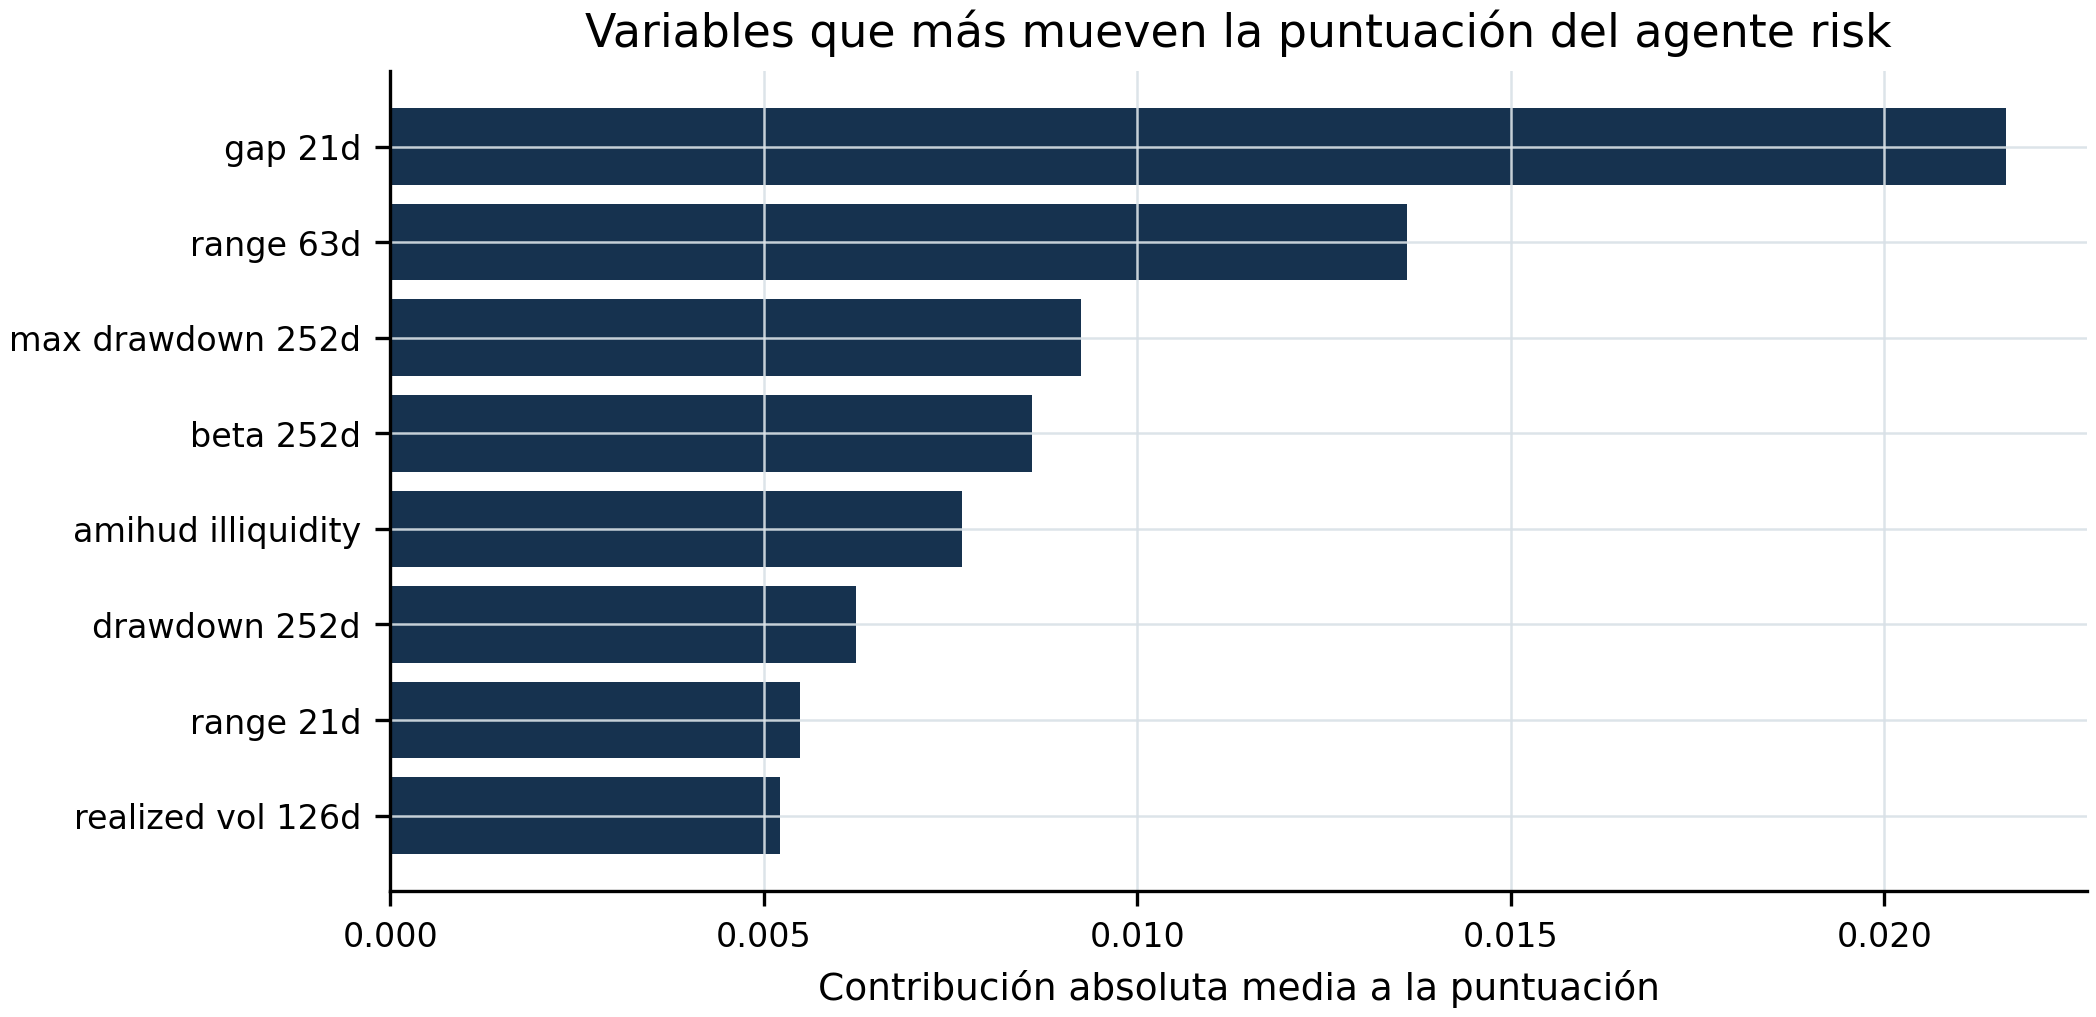
\includegraphics[width=0.92\textwidth]{assets/f05_atribucion_risk.png}
  \caption{Variables que más mueven la puntuación del agente \textit{risk}, por magnitud media de
  contribución local. Fuente: \artefacto{evidence/agent\_local\_attribution.parquet}.}
  \label{fig:atribucion-risk}
\end{figure}

Las dos variables que mandan son \artefacto{gap\_21d} y \artefacto{range\_63d} --- microestructura
del precio a corto plazo: huecos de apertura y amplitud del rango de negociación ---, que juntas
encabezan el 78\,\% de las observaciones. Las medidas que uno esperaría de una estrategia de baja
volatilidad aparecen después y con menos peso: \artefacto{max\_drawdown\_252d} encabeza el 4,2\,\% y
\artefacto{beta\_252d}, el candidato más obvio, ni siquiera está entre las tres primeras. El agente
no está comprando acciones defensivas en el sentido factorial clásico; está leyendo la estructura
reciente de negociación.

Esta observación es coherente con dos resultados independientes del
Capítulo~\ref{chap:resultados}. Explica por qué la neutralización por catorce controles de estilo
retiene el 86,62\,\% de la señal: si el agente dominante replicase el factor de volatilidad, la
neutralización debería destruir mucho más. Y refuerza la advertencia de no reducir el sistema a una
prima conocida, que hasta ahora se sostenía sólo sobre esa neutralización y ahora tiene además una
explicación mecánica.

\begin{figure}[H]
  \centering
  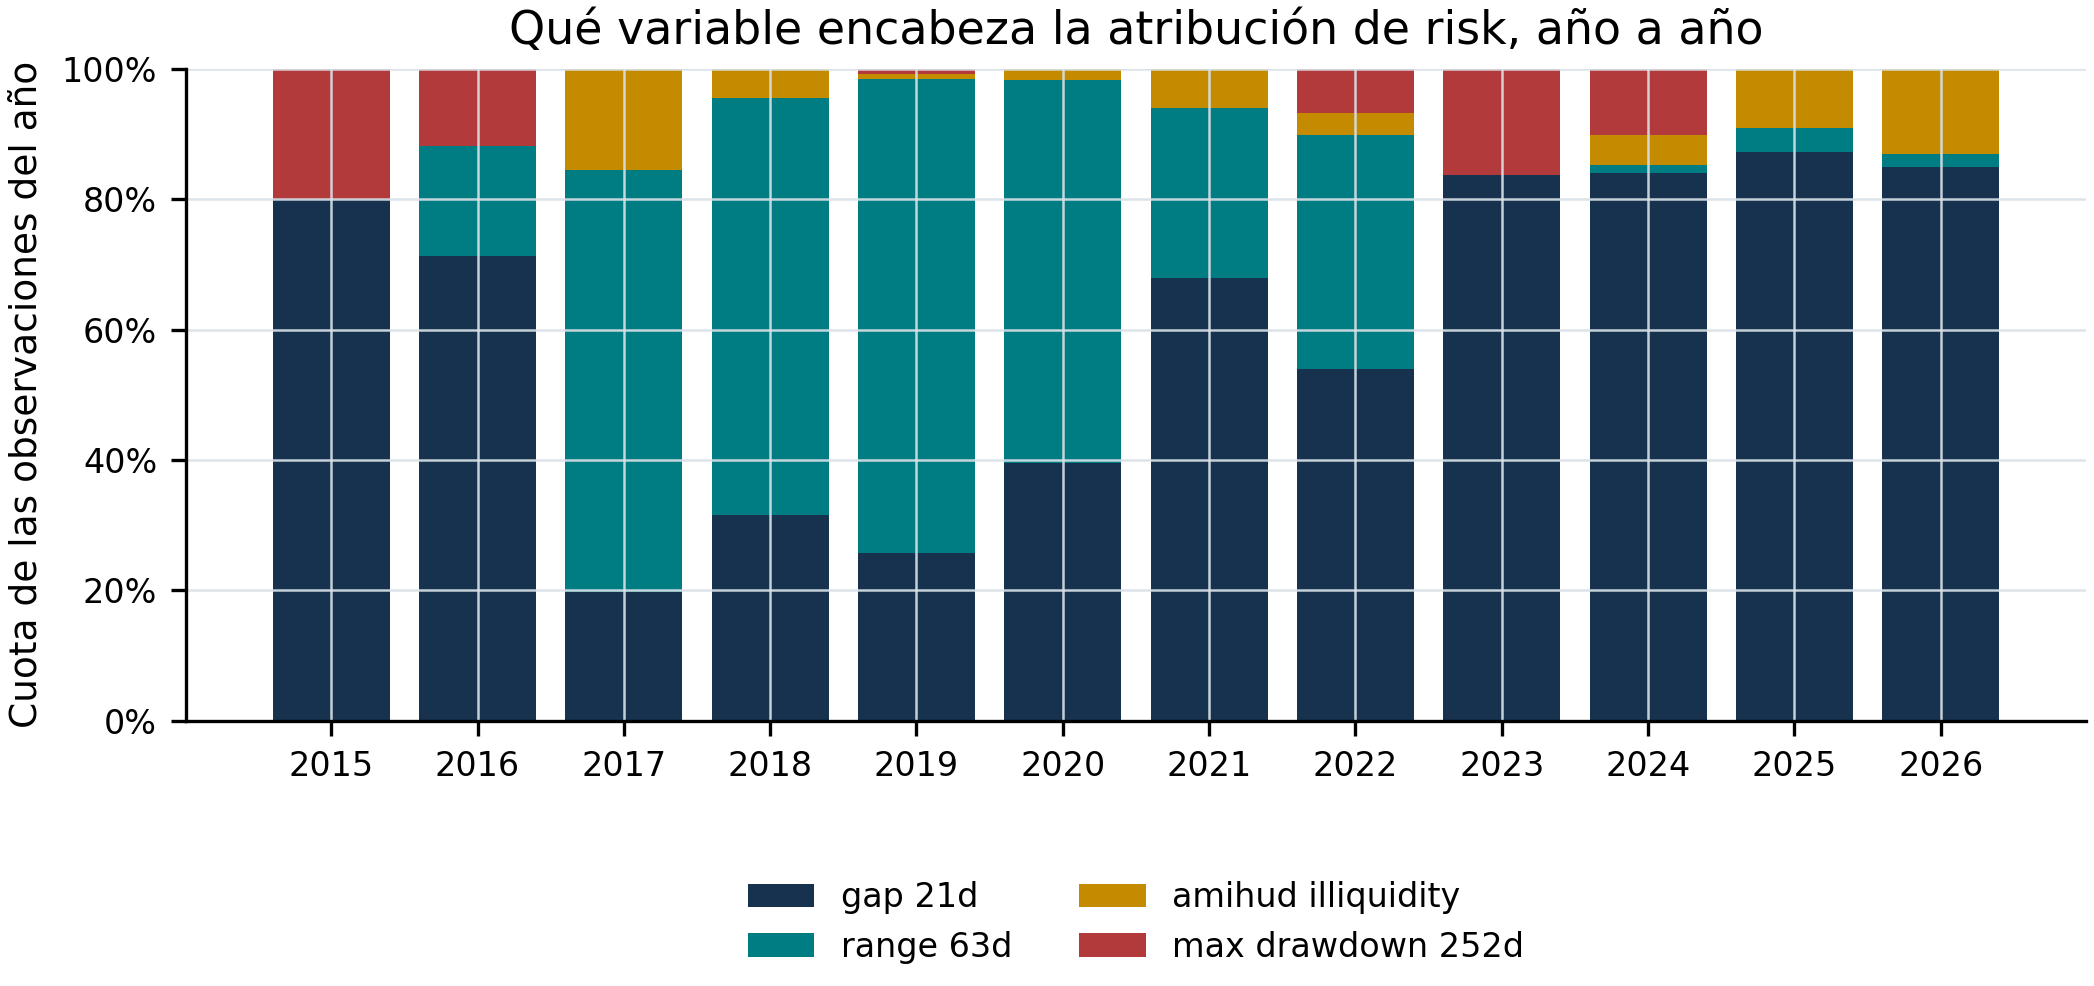
\includegraphics[width=0.92\textwidth]{assets/f05_atribucion_anual.png}
  \caption{Variable que encabeza la atribución de \textit{risk} en cada año, como fracción de las
  observaciones. Fuente: \artefacto{evidence/agent\_local\_attribution.parquet}.}
  \label{fig:atribucion-anual}
\end{figure}

La Figura~\ref{fig:atribucion-anual} añade un matiz importante sobre la concentración del
meta-agente. Aunque \textit{risk} acabe recibiendo más del 95\,\% del peso, no es una apuesta fija:
la variable que lo gobierna cambia con el régimen. \artefacto{range\_63d} domina entre 2017 y 2020
--- el tramo de mayor turbulencia, incluido el desplome de 2020 --- y después se desvanece, mientras
\artefacto{gap\_21d} crece hasta encabezar entre el 64 y el 77\,\% de las observaciones desde 2023. El
sistema reasigna atención dentro del agente aunque el reparto entre agentes esté congelado, lo que
suaviza --- sin eliminarla --- la objeción de que depender de un único especialista equivale a
depender de un único factor.

Conviene declarar el alcance de todo esto. La atribución local es \emph{descriptiva}: dice qué
variables movieron la puntuación, no que esas variables causen el retorno. Ningún contraste de este
capítulo se apoya en ella, y su papel es explicar un resultado ya medido por otros medios, no
sostenerlo.

Una última observación, sobre la amplitud del vocabulario. \textit{Quality} llega a encabezar con
29 variables distintas, casi el triple que \textit{momentum} (10) o \textit{risk} (12), y es a la
vez uno de los peores agentes por Rank-IC (0,0096). No hay aquí evidencia causal --- son cinco
agentes, no una muestra --- pero la asociación es sugerente y apunta en la misma dirección que el
resto del capítulo: repartir la atención entre muchas variables débiles ordena peor que concentrarla
en unas pocas con contenido.

\section{Entrenamiento y combinación de rangos}

En cada snapshot el modelo recibe sólo la historia permitida. Si la fecha es abril de 2020 y la
ventana es de ocho años, el conjunto comienza aproximadamente en abril de 2012; una fila de finales
de 2019 entra sólo si su etiqueta anual ya cerró. El ajuste se repite al avanzar el tiempo. Los
parámetros ganadores ---profundidad 3, 100 estimadores, tasa 0,03 y mínimo de 50 observaciones por
hoja--- limitan interacciones demasiado específicas; se eligieron con la regla del
Capítulo~\ref{chap:diseno-experimental}, no
porque sean universales.

Los scores se convierten a rangos porcentuales dentro de cada cohorte. Esta operación evita que la
escala numérica de un agente domine al resto: si \textit{risk} produce valores entre 0,4 y 0,6 y
\textit{value} entre $-2$ y $3$, ambos pasan a expresar posición relativa en su sección transversal.
El meta combina después esos rangos, no sus unidades originales.

\section{Ejemplo de combinación acotada}

Supóngase una empresa con rangos quality 0,80, value 0,55, growth 0,70, momentum 0,45 y risk 0,90.
En el arranque, los pesos iguales producen $(0,80+0,55+0,70+0,45+0,90)/5=0,68$. Si la evidencia
cerrada concentra el peso en \textit{risk} --- como acaba ocurriendo en la configuración ganadora,
donde ese agente supera 0,95 ---, el score se aproxima a 0,90. La empresa mejora de posición no por
una decisión discrecional, sino porque su fortaleza en \textit{risk} gana relevancia según datos ya
observados. Con la variante libre nada impide esa concentración, y ahí reside tanto su ventaja
medida como el riesgo que se documenta en la sección anterior.

La arquitectura permite atribuir cambios a agentes, no inferir causalidad financiera. Que
\textit{risk} tenga peso alto no demuestra que la baja volatilidad sea la causa del resultado. Puede
reflejar interacciones, características del universo o límites de las variables disponibles. Por eso
los capítulos posteriores muestran estabilidad por eras y neutralización por estilo.
